\chapter{Application Layer}
\section{Principi di applicazioni di rete}
Al cuore di un'applicazione di rete \`e la scrittura di programmi che vengono eseguiti su end systems differenti e comunicano tra di loro attraverso la rete. Per esempio in un'applicazione web ci sono due 
programmi distinti che comunicano tra di loro: il programma browser eseguito sull'host utente e il web server program eseguito nel server host. In P2P file sharing c'\`e un programma in ogni host che partecipa
nella comunit\`a di file-sharing e in questi casi i vari programmi per i diversi host sono simili o identici. Si necessita di scrivere software che sia eseguito su diversi end systems ma non si necessita che giri 
su i dispositivi del network core. 
\subsection{Network application architectures}
L'architettura dell'applicazione di rete \`e creata dallo sviluppatore e determina come \`e strutturata. Ci sono due paradigmi predominanti: client-server e peer-to-peer (P2P).
\subsubsection{Client-server}
In questo paradigma esiste un host sempre attivo chiamato server che conclude richieste da altri host chiamati clients. Nel caso di un web server il server invia oggetti ai clients che poi li visualizzano. In questa
architettura i client non comunicano mai direttamente tra di loro. Il server necessita di un IP fisso e conosciuto in modo che i client possano contattarlo inviando un pacchetto a tale indirizzo. In alcuni casi un 
unico server non basta a gestire tutte le richieste e si utilizza un data center per creare un server virtuale. 
\subsubsection{Peer-to-peer}
In questo paradigma ci si basa minimamente o non ci si basa su server dedicati. Invece l'applicazione utilizza una comunicazione diretta tra host connessi intermittentemente chiamati peers, non posseduti 
da un service provider ma da utenti. Questo paradigma \`e spesso utilizzato in applicazioni a traffico intenso. Esistono approcci ibridi. Una delle caratteristiche pi\`u interessanti \`e la scalabilit\`a: in quanto con 
l'aumento degli utenti aumentano in automatico anche le capacit\`a di comunicazione. Sono inoltre economicamente migliori ma pongono difficolt\`a per quanto riguarda sicurezza, performance e affidabilit\`a.
\subsection{Comunicazione di processi}
Per costruire un'applicazione di rete \`e necessario capire come i programmi comunicano tra di loro. Sono i processi e non i programmi a comunicare tra di loro. Un processo si definisce come un programma che
viene eseguito su un unico end system. Quando processi sono eseguiti sullo stesso end system possono comunicare con comunicazione interprocesso utilizzando regole fornite dal sistema operativo. Processi
su due end system diversi comunicano scambiando messaggi attraverso la rete. Un processo di invio crea un messaggio e lo manda attraverso la rete e un processo di ricezione riceve tali messaggi e 
possibilmente risponde inviandone altri. 
\subsubsection{Processi client e server}
Un'applicazione di rete consiste in paia di processi che inviano messaggi attraverso la rete: per esempio in un'applicazione web un client invia messaggi a un web server process. In un P2P un file \`e trasferito da 
un processo di un peer a un altro peer. Per ogni paio di processi comunicativi si etichetta uno dei due come il client e l'altro come il server. Nel web un browser \`e un processo client e il web server il processo 
server. In P2P il peer che sta scaricando \`e il client e l'altro il server. In alcune applicazioni in processo pu\`o essere sia il client che il server. In ogni caso nel contesto della singola comunicazione assumono 
queste etichette temporaneamente in base al loro ruolo. Si possono pertanto definire come segue: nel contesto di una sessione di comunicazione tra un paio di processi il processo che inizia la comunicazione \`e 
etichettato come il client e il processo che aspetta di essere contattato per iniziare la sessione \`e il server. 
\subsubsection{L'interfaccia tra il processo e la rete}
Come visto sopra la maggior parte delle applicazioni consistono in paia di processi comunicativi con entrambi i processi che si inviano messaggi. Ogni messaggio inviato all'altro deve attraversare la rete 
sottostante. Un processo invia e riceve messaggi dalla rete attraverso un'interfaccia software chiamata socket. Un socket \`e quella parte software che permette al messaggio di uscire dall'end system in modo
da entrare nella rete. Un socket \`e pertanto l'interfaccia tra il layer applicativo e quello di trasporto all'interno di un host. Ci si riferisce a esso anche come l'Application Programming Interface (API) tra 
l'applicazione e la rete in quanto il socket \`e l'interfaccia di programmazione in cui le reti sono costruite. Il solo controllo disponibile da parte dello sviluppatore dell'applicazione sul layer di trasporto \`e la
scelta del protocollo di trasporto e l'abilit\`a di fissare alcuni parametri come il massimo buffer e dimensione dei segmenti. 
\subsubsection{Processi di indirizzamento}
Un processo pu\`o inviare pacchetti unicamente se il processo che li deve ricevere possiede un indirizzo. Per identificare il processo che riceve devono essere specificati il suo indirizzo e un identificatore che 
specifica il processo di ricezione nell'host di destinazione. Nell'internet l'host \`e identificato attraverso il suo indirizzo IP, una quantit\`a a 32 bit che identifica univocamente l'host. Oltre a conoscere l'indirizzo
dell'host si necessita anche di identificare il processo ricevente (ovviamente grazie al suo socket). Questo \`e necessario in quanto un host potrebbe star eseguendo diverse applicazioni di rete. Un port number
di destinazione svolge questo scopo. Applicazioni di vasto utilizzo hanno specifici numeri di porta. Un web server dalla porta 80. un mail server SMTP dal numero 25. 
\subsection{Servizi di trasporto utilizzabili dalle applicazioni}
L'applicazione che invia messaggi spinge messaggi attraverso il socket. Dall'altra parte del socket il protocollo del layer di trasporto ha la responsibilit\`a di portare il messaggio al socket del processo ricevente.
Molte reti mettono a disposizione numerosi protocolli di trasporto e durante lo sviluppo si necessita di sceglierne uno. La scelta dipende dalle caratteristiche necessaria alla singola applicazione.
\subsubsection{Data transfer affidabile}
Essendo che i pacchetti possono andare persi nella rete in caso di corruzione dei bit o overflow dei buffer e che per molte applicazioni la perdita dei dati pu\`o avere conseguenze devastanti per supportare queste
applicazioni si deve garantire che i dati inviati siano ricevuti correttamente e completamente. Se un protocollo garantisce questo \`e detto che provvede ad un reliable data transfer. La perdita per alcune 
applicazioni pu\`o essere tollerata (loss-tolerant applications) come quelle di invio di multimedia. 
\subsubsection{Throughput}
Il throughput \`e il tasso al quale il processo di invio pu\`o inviare dati al processo di ricezione. In quanto altre sessioni andranno a condividere la bandwidth lungo il percorso di rete il throughput pu\`o variare 
con il tempo. Queste osservazioni portano ad un altro servizio che un protocollo di trasporto deve poter provvedere: ovvero una garanzia di throughput a uno specifico tasso. L'applicazione pu\`o garantire un 
throughput di almeno $r\frac{bits}{sec}$. Queste applicazioni sono dette bandwidth-sensitive application e sono per esempio quelle di multimedia, anche se possono utilizzare tecniche di encoding adattive
per sfruttare il throughput variabile. Elastic application invece non necessitano di un throughput stabile, semplicemente funzionano pi\`u velocemente maggiore \`e il throughput. 
\subsubsection{Timing}
Un protocollo di trasporto pu\`o mettere a disposizione garanzie di tempo, maggiormente utilizzate per applicazioni real-time, ad esempio attraverso constraints di limite superiore al ritardo dei bit. 
\subsubsection{Security} 
Un protocollo di trasporto pu\`o mettere a disposizioni applicazioni con uno o pi\`u servizi di sicurezza attraverso criptazione dei dati all'invio e decriptazione alla ricezione. 
\subsection{Servizi di trasporto dell'internet}
L'internet e reti TCP/IP mettono a disposizioni due protocolli di trasporto: UDP e TCP.  Nessuno dei due \`e criptato.
\subsubsection{TCP services}
TCP include un servizio connection-oriented e reliable data transfer. Quando un'applicazione invoca TCP come protocollo di trasporto riceve:
\begin{itemize}
\item Connection-oriented service: TCP fa in modo che client e server scambino informazioni di controllo transport-layer tra di loro prima che il messaggio dell'application layer cominci a fluire. Questo 
handshaking permette ai due di prepararsi per l'arrivo dei pacchetti. Dopo la fase di handshaking una connessione TCP esiste tra i socket dei due processi. La connessione \`e full-duplex in quanto 
entrambi i processi possono sia ricevere che inviare pacchetti. Quando l'applicazione termina di inviare messaggi deve distruggere la connessione.
\item Reliable data transfer service: il processo di comunicazione pu\`o basarsi su TCP per inviare i dati senza errori e nell'ordine giusto. 
\end{itemize}
TCP possiede anche un meccanismo di congestion-control che throttles (rallenta) un processo di invio quando la rete tra inviante e ricevente \`e congestionata. Per permettere la criptazione e la sicurezza
si aumenta il TCP trasformandolo nell'SSL (Secure Sockets Layer) che passa i dati in chiaro al socket SSL che li cripta e li invia al TCP socket. Vengono poi ricevuti dal TCP socket che li passa a quello SSL che li
decripta.
\subsubsection{UDP sevices}
UDP \`e un protocollo di trasporto leggero che mette a disposizione servizi minimali: \`e senza connessione e non c'\`e l'handshaking prima che i due processi inizino a comunicare. Provvede un data tranfer 
service non affidabile e i pacchetti potrebbero arrivare in disordine. Non include un meccanismo di controllo della congestione. 
\subsubsection{Servizi non messi a disposizione}
Si noti come nell'internet non esistono servizi per garantire throughput e temporizzazione. Nonostante questo applicazioni real time riescono a funzionare grazie a un design attento e specializzato.
\subsection{Protocolli application-layer}
Un protocollo di application-layer definisce come un processo dell'applicazione eseguito su diverse macchine invia messaggi agli altri, definisce:
\begin{itemize}
\item Il tipo di messaggi scambiati.
\item La sintassi dei tipi di messaggio come i campi nel messaggio e come sono delineati.
\item La semantica dei campi, il significato dell'informazione contenuta in essi.
\item Regole per determinare quando e come un processo invia e risponde a messaggi.
\end{itemize}
Alcuni di questi protocolli sono specificati in RFCs e sono di dominio pubblico come HTTP. Se uno sviluppatore di browser segue le regole dell'RFC dell'HTTP il browser sar\`a capace di recuperare pagine web
da un qualsiasi server web che segue le regole dell'HTTP RCF. Esistono anche protocolli proprietari e non i dominio pubblico. 
\section{Il Web e HTTP}
Il web opera on demand: gli utenti ricevono cosa vogliono quando lo vogliono. 
\subsection{Panoramica di HTTP}
L'HyperText Transfer Protocol (HTTP) \`e il protocollo del livello di applicazione del Web. \`e definito nel RFC 1945 e RFC 2616. \`E implementato in due programmi: uno client e uno server. Il programma client
e server sono eseguiti su due end systems diversi e comunicano attraverso messaggi HTTP. HTTP definisce la struttura di questi messaggi e come client e server li scambiano. Si definisce una Web page
o documento come costituita da oggetti. Un oggetto \`e un file che \`e indirizzabile attraverso un singolo URL. La maggior parte delle pagine Web consistono in un file HTML di base e molti oggetti referenziati.
Ogni URL presenta due componenti: l'hostname del server che contiene l'oggetto e il nome del percorso dell'oggetto. Server Web che implementano il lato server dell'HTTP contengono Web object ognuno
indirizzabile attraverso un URL. HTTP definisce come Web clients richiedono Web pages da Web servers e come questi trasferiscono Web pages ai clients. Quando un utente richiede una Web page il browser
invia un messaggio di richiesta HTTP per l'oggetto nella pagina al server. Il server riceve la richiesta e risponde con un messaggio di risposta HTTP che contiene gli oggetti. HTTP utilizza TCP come protocollo di
trasporto sottostante. Il client HTTP inizia una connessione TCP con il server. Una volta che la connessione \`e stabilita i processi browser e server accedono al TCP attraverso le interfacce socket. Un client invia
un messaggio di richiesta HTTP nell'interfaccia socket e riceve messaggi di risposta HTTP dalla sua interfaccia socket. Il processo \`e analogo per i server. \`E importante notare come il server invia file richiesti
ai clients senza salvare alcuna informazione sullo stato di essi. Per questo motivo si dice che HTTP \`e uno stateless protocol e il Web utilizza l'architettura client-server. Un Web server \`e sempre acceso
con un IP fisso.
\subsection{Connessioni persistenti e non persistenti}
In molte applicazioni internet il client e il server comunicano per un periodo esteso con il client con quest'ultimo che fa una serie di richieste e il server che risponde ad ognuna di esse. In base all'applicazione
e a come viene usata la serie di richieste pu\`o essere utilizzata back-to-back, periodicamente o a intermittenza. Quando questa interazione si svolge attraverso TCP si deve decidere se ogni richiesta risposta 
debba essere fatta attraverso una connessione TCP separata o sulla stessa connessione. Nel primo approccio l'applicazione utilizza una connessione non persistente, mentre nel secondo persistente. 
Nonostante HTTP utilizza di default connessioni persistenti, client e server possono essere configurati in modo da utilizzare quella non persistente.
\subsubsection{Round-trip time}
 Si definisce round-trip time (RTT) il tempo che impiega un pacchetto a viaggiare da un client a un server e ritornare al client. RTT include packet-propagation delays, packet-queuing delays. e packet-processing 
 delays. 
\subsubsection{HTTP con connessione non persistente}
Si elenchino ora i passi necessari per trasferire una web page da server a client nel caso di connessione non persistente. Si supponga che la pagina consista di un HTML base contenente $N$ file referenziati e 
che questi si trovino sullo stesso server.
\begin{enumerate}
\item Il client HTTP inizia una connessione TCP con il server sulla porta $80$. Associata alla connessione ci sar\`a un socket al client e uno al server.
\item Il client HTTP invia un messaggio di richiesta HTTP attraverso il suo socket che include il percorso del file.
\item Il processo server HTTP riceve il messaggio dal socket, recupera l'oggetto dalla memoria, lo incapsula in un messaggio di risposta HTTP e invia il messaggio di risposta al client attraverso il suo socket.
\item Il processo server HTTP indica a TCP di chiudere la connessione e TCP aspetta che il client abbia ricevuto la risposta intatta prima di chiudersi.
\item Il client HTTP riceve il messaggio di risposta, la connessione TCP termina. Il messaggio indica che l'oggetto incapsulato \`e un file HTML, lo estrae dal messaggio, lo esamina e verifica che referenzia gli
$N$ oggetti.
\item I primi quattro passaggi sono ripetuti per gli $N$ oggetti referenziati.
\end{enumerate}
Quando il browser riceve la pagina la mostra all'utente. Due browser diversi potrebbero interpretarla in modo diverso in quanto le specifiche HTTP definiscono unicamente il protocollo di comunicazione. 
L'apertura delle diverse connessioni TCP pu\`o essere fatta in maniera parallela. Quando si vuole richiedere una Web page si apre una connessione TCP, che la conferma con un altro messaggio e il client 
riconferma. Le prime due parti richiedono un RTT. Dopo aver completato l'handshaking il client invia un messaggio di richiesta HTTP combinato con la terza parte dell'handshake e una volta che arriva al server
questo invia l'HTML file nella connessione TCP. Questa richiesta risposta HTTP richiede un altro RTT. Pertanto il tempo di risposta totale \`e due RTT pi\`u il tempo di trasmissione al client del file HTML.
\subsubsection{HTTP con connessione persistente}
Con questo tipo di connessione il server lasca aperta la connessione TCP dopo aver inviato la risposta. Richieste successive dallo stesso client possono essere inviata dalla stessa connessione. Queste richieste
possono essere fatte back-to-back senza aspettare per le rispose di richieste in fase di elaborazione (pipelining). Tipicamente il server HTTP chiude una connessione dopo un intervallo di tempo. E quando riceve
richieste back-to-back invia oggetti back-to-back. L'HTTP di default utilizza connessioni persistenti con pipelining. HTTP/2 permette richieste multiple sulla stessa connessione. 
\subsection{Formato dei messaggi HTTP}
Esistono due tipi di messaggio HTTP: richiesta e risposta.
\subsubsection{Messaggio di richiesta HTTP}
Un messaggio HTTP \`e scritto in testo ASCII e consiste di un numero arbitrario di righe, ognuna seguita da un carriage return e un line feed. L'ultima riga \`e seguita da un carriage return e un line feed 
addizionale. La prima riga \`e chiamata la request line e quelle seguenti header lines. Le request line hanno tre campi: il campo di metodo, il campo URL e il campo di versione HTTP. Il metodo pu\`o avere
valori diversi come \emph{GET, POST, HEAD, PUT, DELETE}. La maggior parte delle richieste utilizzano il metodo \emph{GET}, utilizzato quando il browser richiede un oggetto identificato dall'URL. L'header
contiene informazioni riguardo l'host: \emph{Host: }, il tipo di connessione (persistente o non persistente) \emph{Connection: }, il tipo di browser che sta facendo la richiesta: \emph{User-agent: } e il linguaggio
preferito dall'utente: \emph{Accept-language: }. Il metodo \emph{POST} \`e utilizzato quando l'utente completa un form. Dipendentemente dal valore inserito dall'utente l'entity body contiene quel dato. Si 
pu\`o utilizzare anche il \emph{GET} in questi casi ma i dati sono salvati nell'URL: \emph{URLsearch?field1\& field2\&$\dots$\& fieldn}. Il metodo \emph{HEAD} \`e simile al \emph{GET} ma non ritorna 
l'oggetto richiesto. Il metodo \emph{PUT} permette all'utente di caricare un oggetto su un percorso specifico. Il metodo \emph{DELETE} permette di eliminare un oggetto.
\begin{figure}
\includegraphics[width=\textwidth]{Pictures/HTTPRequestMessage.png}
\caption{Forma generale di un messaggio di richiesta HTTP}
\end{figure}
\subsubsection{Messaggio di risposta HTTP}
Il messaggio \`e composto di tre sezioni: un'iniziale status line, delle header line e un entity boy. L'entity body contiene l'oggetto richiesto. La status line ha tre campi: il campo della versione del protocollo, un
codice di status, e il corrispondente messaggio di stato.  Le header line contengono il tipo di connessione \emph{Connection: }, il tempo e la data in cui la risposta HTTP \`e stata creata \emph{Date: }, il tipo di 
server utilizzato \emph{Server: }, il tempo dell'ultima modifica al file \emph{Last-Modified: } critica per l'object-caching, il numero di bit della risposta: \emph{Content-Length: }, il tipo di oggetto nell'entity 
body \emph{Content-Type: }. Il codice di stato pu\`o contenere questi valori:
\begin{itemize}
\item \emph{200 OK}: la richiesta ha avuto successo.
\item \emph{301 Moved Permanently}: l'oggetto richiesto \`e stato mosso permanentemente e il nuovo URL \`e specificato in \emph{Location: } nell'header. Il software client lo recupera automaticamente.
\item \emph{400 Bad Request}: la richiesta non \`e stata compresa dal server.
\item \emph{404 No Found}: il documento richiesto non esiste sul server.
\item \emph{505 HTTP Version Not Supported}: la versione del protocollo HTTP richiesta non \`e supportata dal server.
\end{itemize}
\begin{figure}
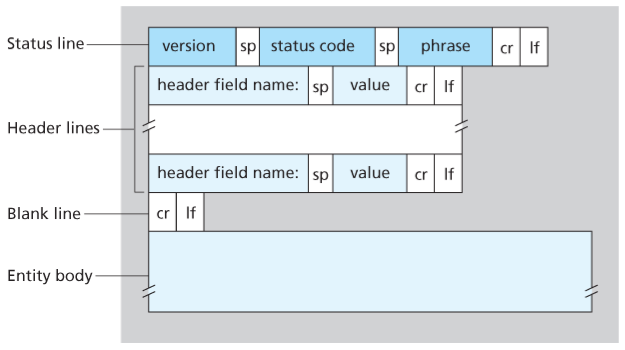
\includegraphics[width=\textwidth]{Pictures/HTTPResponseMessage.png}
\caption{Forma generale di un messaggio di risposta HTTP}
\end{figure}
\subsection{Interazioni utente-server: Cookies}
HTTP \`e stateless in modo da permettere Web server con alte performance e in grado di gestire migliaia di connessioni TCP simultanee. Si rende per\`o desiderabile identificare utenti. Per questo motivo 
vengono utilizzati cookies che permettono di tenere traccia degli utenti. La tecnologia cookie ha quattro componenti: un header line nel messaggio HTTP di risposta, un header nel messaggio di richiesta HTTP, 
un file cookie tenuto sull'end system utente e gestito dal browser e un database back-end sul web site. Quando si compie un primo accesso ad un Web server si crea un numero unico di identificazione e crea 
un entry nel database indicizzato su quel numero. Il server poi risponde al browser includendo nella risposta HTTP \emph{Set-cookie:} che contiene il numero di identificazione. Quando il browser legge questa
linea appende una riga al cookie file che gestisce che include l'hostname e il numero di identificazione. Per gli accessi seguenti nell'header viene messo un cookie header che include il numero identificativo. 
\subsection{Web Caching}
Una Web cache o proxy server \`e un entit\`a della rete che soddisfa richieste HTTP al posto del web server originario. La cache possiede il proprio spazio di archiviazione che contiene copie di oggetti 
recentemente richiesti. Un browser pu\`o essere configurato in modo da tutte le richieste HTTP passino prima per la cache. Se questa non possiede il file inoltra la richiesta al server originario salvandola e 
poi inviandola all'utente. La cache \`e contemporaneamente un server e un client. Vengono utilizzate per aumentare la bandwidth e per ridurre il traffico verso i web server. Le web caches stanno prendendo un 
ruolo sempre pi\`u importante grazie a Content Distribution Networks (CDNs): una compagnia di CDN installa molte caches geograficamente distribuite localizzando il traffico. 
\subsubsection{Il GET condizionale}
Nonostante il caching possa ridurre il tempo di risposta percepito pu\`o introdurre il problema del controllo delle versioni dei file salvati in essa. Esiste un meccanismo in HTTP per permettere alla cache se i 
suoi file sono up-to-date: il \emph{GET} condizionale. Un get condizionale utilizza il metodo \emph{GET} e inserisce nell'header la linea \emph{If-modified-Since} il cui valore \`e nello stesso formato della
linea \emph{Last-modified}.
\section{Electronic mail}
E-mail \`e un mezzo di comunicazione asincrono veloce, facile da distribuire ed economico. Ogni utente possiede una mailbox locata in uno dei mail servers che mantiene e gestisce i messaggi che sono inviati
all'utente. Un messaggio tipico inizia nell'user agent del mittente e viaggia fino alla mail server del ricevente dove \`e depositata nella sua mailbox. Quando un utente vuole accedere ad un messaggio il mail 
server contenente la mailbox lo autentica. Se il server di spedizione non pu\`o inviare il messaggio nel server del ricevente il messaggio viene mantenuto un una message queue e prova a trasferire il messaggio 
pi\`u tardi. Ogni tentativo \`e fatto indicativamente ogni 30 minuti. Se non c'\`e successo dopo molti giorni il server rimuove il messaggio e notifica il mittente. SMTP \`e il protocollo application-layer principale. 
Utilizza TCP. SMTP ha due lati: lato client che viene eseguito sul mail server del mittente e un lato server eseguito sul mail server del ricevente. Entrambi i lati sono eseguiti su ogni mail server. 
\subsection{SMTP}
SMTP trasferisce i messaggi. Essendo molto precedente all'HTTP possiede certe caratteristiche arcaiche. Quando si invia un messaggio:
\begin{enumerate}
\item Il mittente invoca il suo user agent per e-mail, inserisce l'indirizzo e-mail del ricevente, compone un messaggio e dice all'user agent di inviarlo.
\item L'user agent del mittente invia il messaggio al suo mail server dove \`e posto in una message queue.
\item Dopo un SMTP handshaking iniziale il client SMTP invia il messaggio nella connessione TCP.
\item Al mail server del ricevente il lato server di SMTP riceve il messaggio e il mail server lo posiziona nella mail box del ricevente.
\item Il ricevente invoca il suo user agent per leggere il messaggio secondo la sua convenienza.
\end{enumerate}
SMTP solitamente non utilizza mail server intermedi. Per inviare i messaggi il client SMTP stabilisce una connessione alla porta 25 al server SMTP. Una volta che la connessione \`e stabilita si svolgono degli 
handshaking. Durante questa fase il client indica l'indirizzo e-mail del mittente e del ricevente. Dopo questa fase il client invia il messaggio. Il client successivamente ripete il processo sulla stessa connessione 
TCP se deve inviare altri messaggi altrimenti chiude la connessione. In un messaggio SMTP le righe con prefisso \emph{C:} sono le righe che il client invia nel socket TCP e quelle con prefisso \emph{S:} sono
quelle inviate dal server. Durante la comunicazione il client invia cinque comandi: \emph{HELO} seguito dal proprio mail server, \emph{MAIL FROM:} in cui \`e indicato l'indirizzo e-mail del mittente, 
\emph{RCPT TO:} dove \`e indicato l'indirizzo del ricevente \emph{DATA} contenenti il corpo dell'e-mail terminato da una singola riga contenente un punto e \emph{QUIT} per terminare la connessione. SMTP
utilizza connessioni persistenti. La prima riga contiene l'avvenuta connessione con il server del ricevente con il codice \emph{220}.
Per messaggi multimediali viene utilizzata l'estensione di SMTP MIME. 
\subsection{Comparazione con HTTP}
HTTP \`e primariamente un protocollo di pull, in particolare la connessione TCP \`e inizializzata dalla macchina che vuole ricevere il file. SMTP \`e primariamente un push protocol in quanto la connessione TCP 
\`e iniziata dalla macchina che vuole inviare i file. SMTP inoltre richiede che ogni parte del messaggio, compreso il corpo sia nello standard ASCII a 7 bit. Inoltre HTTP incapsula ogni oggetto in un diverso
messaggio HTTP, mentre in SMTP posiziona ogni oggetto del messaggio nel messaggio stesso.
\subsection{Formato dei messaggi mail}
Quando un messaggio e-mail \`e inviato informazioni secondarie sono contenute in una serie di righe header definite in RFC 5322 che ne specifica il formato esatto. Ogni riga header contiene testo leggibile che
consiste in parole chiave seguite dai due punti e un valore. Ogni header deve posseder un \emph{From:} e un \emph{To:}, pu\`o includere un \emph{Subject:}. Dopo l'header segue una riga vuota e il corpo del
messaggio. 
\subsection{Protocolli di accesso Mail}
Dopo che SMTP consegna il messaggio nel mail server e questo \`e posizionato nella mailbox del ricevente che lo visualizza attraverso un client. Solitamente le mailbox si trovano in mail server condivisi. Per 
accedere ai propri messaggi un protocollo speciale di accesso mail trasferisce i messaggi dal mail server all'end system del ricevente. Ne esistono vari tra cui Post Office Protocol-Version 3 (POP3), Internet
Mail Access Protocol (IMAP) e HTTP.
\subsubsection{POP3}
POP3 \`e definito nel RFC 1939 ed \`e semplice e con poche funzionalit\`a. POP3 comincia quando l'user agent apre una connessione TCP con il mail server sulla porta 110. Dopo averla aperta POP3 prosegue 
con l'autorizzazione, transazione e aggiornamento. Durante la prima fase l'user agent invia uno username  e una password in chiaro per autentificare l'utente. Durante la seconda fase l'user agent recupera i
messaggi e pu\`o marcarli per eliminazione e ottenere le statistiche della mail. La terza fase accade dopo il comando \emph{quit} che finisce la sessione POP3 e durante questa fase il mail server elimina i 
messaggi marcati per eliminazione. In una transazione POP3 l'user agent invia comandi e il server risponde con una risposta. Ce ne sono due possibili: \emph{+OK} seguita da dati server-to-client per indicare
il successo del comando e \emph{-ERR} usato dal server per indicare un errore con il comando. La fase di autorizzazione ha due comandi principali: \emph{user $<$username$>$} e \emph{
pass $<$password$>$}.  Durante la fase di transazione un user agente POP3 pu\`o essere configurato dall'utente per scaricare ed eliminare o scaricare e mantenere. La sequenza di comandi inviati dipende
da quale di questi due modelli viene utilizzato. Nel primo l'user agent invia il comando \emph{list, retr, dele}. POP3 \`e stateless.
\subsubsection{IMAP}
Con accesso POP3 il ricevente scarica i suoi messaggi sulla macchina locale, pu\`o creare cartelle mail e spostare mail scaricate in cartelle, cercare per messaggi. Questo paradigma pone un problema per 
un utente nomade che preferirebbe utilizzare una gerarchie di cartelle su un server remoto che pu\`o essere acceduto da ogni computer. Per risolvere questo problema nel RFC 3501 viene definito il protocollo 
IMAP. Possiede molte pi\`u capacit\`a del POP3 ma \`e anche significativamente pi\`u complesso. Un server IMAP associa ogni messaggio con una cartella e quando un messaggio arriva al server \`e associato 
con la cartella INBOX del ricevente che potr\`a poi spostarlo in una nuova cartella, leggerlo, eliminarlo, eccetera. Mette a disposizione comandi per permettere agli utenti di creare cartelle e spostare messaggi
da una all'altra e per cercare cartelle remote che corrispondono a criteri specifici. Un server IMAP mantiene informazioni sullo stato degli utenti. Inoltre possiede comandi che permettono agli user agent di
ottenere componenti dei messaggi. Per facilitare connessioni con bandwidth basso. 
\subsubsection{Web-Based E-Mail}
Con questo servizio l'user agent \`e un ordinario Web browser che comunica con la mailbox attraverso HTTP. 
\section{DNS - Internet's Directory Service}
Gli host dell'internet sono identificati da un hostname human readable e un indirizzo IP composto da quattro byte rappresentati
attraverso una dotted decimal notation che fornisce informazioni sulla posizione relativa dell'host nell'internet.
\subsection{Servizio di un DNS}
Per tradurre un hostname nel corrispondente indirizzo IP si crea un servizio di directory. Il ruolo principale del domain name system dell'internet \`e questo. Il DNS \`e un database distribuito implementato in
una gerarchia di server DNS e un protocollo di livello applicativo che  permette agli host di fare query su questo database. I server DNS sono macchine UNIX che eseguono il software Berkeley Internet Name 
Domain (BIND). Il protocollo DNS esegue UDP e usa la porta 53. \`E comunemente utilizzato da altri protocolli application layer come HTTP e SMTP per tradurre hostname in indirizzi IP:
\begin{enumerate}
\item La stessa macchina utente viene eseguita sul lato client di un'applicazione DNS.
\item Il browser estrae l'hostname dall'URL e lo passa al lato client dell'applicazione DNS.
\item Il lato client del DNS invia una query contenente l'hostname al server DNS.
\item Il client DNS riceve una risposta che contiene l'indirizzo IP corrispondente.
\item Una volta che il browser riceve l'indirizzo IP pu\`o iniziare una connessione TCP.
\end{enumerate}
Il DNS aggiunge un ritardo ulteriore alle applicazioni che lo utilizzano. Spesso gli indirizzi IP sono cachati in un DNS server locale in modo da ridurre il traffico verso i server DNS. Provvedono inoltre altri servizi:
\begin{itemize}
\item Host aliasing: un host con un nome complicato pu\`o avere uno o pi\`u alias. Il primo \`e detto hostname canonico.
\item Mail server aliasing. 
\item Load distribution: il DNS \`e utilizzato per distribuire il carico tra i server replicati. Quando siti sono replicati su diversi indirizzi IP il DNS invia tutta la lista ma ruota l'ordine degli indirizzi con ogni risposta. 
\`E utilizzato anche per i mail server.
\end{itemize}
Il DNS \`e specificato negli RFC 1034 e RFC 1035 e aggiornato in molti altri.
\subsection{Funzionamento del DNS}
Un design semplice per il DNS avrebbe un server DNS che contiene tutte le mappature da hostname a IP. \`E impraticabile in quanto:
\begin{itemize}
\item Possiede un singolo punto di fallimento.
\item Dovrebbe sostenere un volume di traffico immenso.
\item Il database centralizzato potrebbe essere troppo distante e pertanto introdurre un ritardo notevole.
\item Richiederebbe aggiornamenti troppo frequenti per ogni nuovo host.
\end{itemize}
Questo design fallisce in quanto non riesce a scalare. Per questo il DNS \`e distribuito.
\subsubsection{Un database distribuito e gerarchico}
Per gestire i problemi di scala il DNS utilizza un gran numero di server organizzati gerarchicamente e distribuiti geograficamente. Nessun server DNS contiene tutte le mappature. Ad una prima 
approssimazione esistono tre classi di DNS: server DNS radice, top-level domain (TLD) DNS e authoritative. Il client contatta la radice che ritorna l'IP di un TLD secondo l'ultimo dominio (.com) che a sua volta
ritorna un IP di un DNS authoritative. Oltre a questi esistono server DNS locali che non appartengono alla gerarchia ma si comportano da proxy per le richieste agli altri DNS. Una query DNS pu\`o essere 
iterativa (il DNS locale comunica solo con il DNS radice) o ricorsiva (il DNS locale comunica con tutti i DNS necessari). 
\subsubsection{DNS caching}
In una catena di query quando un DNS server riceve una risposta pu\`o cachare la mappatura nella sua memoria locale. Essendo host e mappature non permanenti le informazioni cachate sono scartate dopo un
periodo, tipicamente due giorni. 
\subsection{DNS records e messaggi}
I server DNS che implementano il database distribuito DNS salvano resource records (RRs) che includono quelli che forniscono la mappatura hostname-to-IP. Ogni messaggio di risposta DNS contiene
uno o pi\`u RRs. Un resource record \`e una tupla che contiene i campi \emph{(Name, Value, Type, TTL)}. \emph{TTL} \`e il tempo che rimane al RR e determina quando dovrebbe essere rimosso dalla cache. 
Il significato di \emph{Name} e \emph{Value} dipende da \emph{Type}:
\begin{itemize}
\item Se \emph{Type=A} allora \emph{Name} \`e un hostname e \emph{Value} \`e l'indirizzo IP. 
\item Se \emph{Type=NS} allora \emph{Name} \`e un dominio e \emph{Value} \`e l'hostname di un server authoritative DNS che sa come ottenere l'indirizzo IP.  \`E utilizzato per instradare query DNS lungo
la query chain.
\item Se \emph{Type=CNAME} allora \emph{Value} \`e l'hostname canonico per l'hostname halias \emph{Name}.
\item Se \emph{Type=MX} allora \emph{Value} \`e il nome del mail server canonico che ha un alias hostname \emph{Name}. 
\end{itemize}
Se un server DNS \`e authoritative per un particolare hostname contiene un record \emph{Type=A} per quell'hostname. Se non lo \`e contiene un record \emph{Type=NS} e uno \emph{Type=A} per il server 
DNS nel campo \emph{Value} del primo.
\subsubsection{Messaggi DNS}
Esistono due tipi di messaggio DNS: query e risposta e hanno lo stesso formato. 
\begin{itemize}
\item I primi 12 byte nella sezione header contengono vari campi:
\begin{itemize}
\item Il primo campo \`e un numero a 16 bit che identifica la query. \`E copiato nel messaggio di risposta in modo di verificare la corrispondenza tra query inviate e risposte ricevute.
\item Flags che indicano se il messaggio \`e una query o una risposta, una flag \`e settata in risposta se il DNS \`e authoritative, un altra se si desidera compiere della ricorsione, la cui disponibilit\`a \`e controllata
da un'altra. 
\item Quattro campi number-of che indicano il numero di occorrenze dei quattro tipi di sezioni dati che seguono l'header.
\end{itemize}
\item La question section contiene informazioni riguardanti la query che si sta svolgendo: include un campo di nome che contiene il nome che si sta richiedendo, un campo tipo che indica il tipo di domanda 
riguardo il nome.
\item In una risposta da un server DNS l'answer section contiene gli RRs per il nome che era stato originariamente richiesto che possono essere multipli.
\item L'authority section contiene records di altri servers authoritative.
\item L'additional section contiene altri record utili.
\end{itemize}
\subsubsection{Inserire records nel database DNS}
Esiste un registrar, un'entit\`a commerciale che verifica l'unicit\`a del nome di dominio, lo inserisce in un database DNS. Si devono fornire i nomi e indirizzi IP dei server DNS authoritative primari e secondari. Per ognuno di questi server authoritative il registrar fa in modo che record di tipo A e NS
siano registrati nei server TLD. E si deve fare attenzione ad inserire nel proprio server record di tipo A per il web server e di tipo MX per il mail 
server.
\section{Distribuzione di file Peer-to-Peer}
In un'architettura P2P esiste una minima o nessuna dipendenza verso un sistema centrale sempre attivo: intermittenetemente paia di hosts connessi detti peers 
comunicano direttamente tra di loro. Questi peers sono macchine controllate/possedute dagli utenti. Si consideri una naturale applicazione del P2P: la
distribuzione di file attraverso un protocollo detto bitTorrent in cui ogni peer pu\`o inviare una parte del file richiesto in modo da diminuire il carico
sul sistema centrale.
\subsection{Scalabilit\`a di architetture P2P}
Per considerare la naturale scalabilit\`a delle architetture P2P si consideri un modello di distribuzione file: si denoti il tasso di upload dell'access 
link del server con $u_s$, quello dell'i-esimo peer con $u_i$ e il tasso di download dell'i-esimo peer con $d_i$. Si indichi con $F$ la dimensione in bit
del file da distribuire e con $N$ il numero di peer a cui verr\`a distribuito tale file. Si intender\`a con tempo di distribuzione il tempo che verr\`a 
impiegato per distribuire il file a tutti i peers. 
\paragraph{Tempo di distribuzione client-server}
Si determini prima il tempo di distribuzione per le architetture client-server denotato con $D_{cs}$. Si 
osserva come il server deve distribuire completamente una copia ad ognuno degli $N$ peers e deve pertanto trasmettere $NF$ bits. Pertanto impiegher\`a 
$\frac{NF}{u_s}$ tempo. Sia ora $d_{\min}$ il tasso di download minimo tra i peers. Tale peer non potr\`a ricevere il file prima di $\frac{F}{d_{\min}}$. 
Attraverso queste osservazioni si nota come $D_{cs}=\max(\frac{NF}{u_s}, \frac{F}{d_{\min}})$. Si nota pertanto che il tempo di distribuzione cresce 
linearmente con il numero di peers $N$. 
\paragraph{Tempo di distribuzione P2P}
Calcolando il tempo di distribuzione per le architetture P2P si nota come un peer pu\`o assistere il server nell'invio dei dati utilizzando la propria 
capacit\`a di upload per inviarlo ad altri peers. Si consideri come all'inizio della distribuzione solo il server possiede il file. Per riuscire a inviare 
il file nella comunit\`a dei peers deve inviarlo almeno una volta attraverso il proprio access link, pertanto il tempo minimo \`e $\frac{F}{u_s}$. Il peer
con il tasso di download pi\`u basso non lo potr\`a ottenere prima di $\frac{F}{d_{\min}}$, rendendolo di fatto il tempo minimo. Si osservi come la 
capacit\`a di upload del sistema sia pari alla capacit\`a di upload del server e di tutti i peers, pertanto $u_{total}=u_s+u_0+\cdots u_N$. Tale sistema 
deve distribuire il file $F$ a tutti $N$ i peers, pertanto il tempo di distribuzione sar\`a $\frac{NF}{u_s+u_0+\cdots u_N}$. Unendo queste considerazioni si 
noti come il tempo di distribuzione diventa $D_{P2P}=\max\{\frac{F}{u_s}, \frac{F}{d_{\min}}, \frac{NF}{u_s+\sum\limits_{i=1}^Nu_i}\}$. Questo tempo non 
diventa pi\`u lineare con il numero di peers e pertanto provvede una scalabilit\`a implicita.
\subsection{BitTorrent}
BitTorrent \`e un popolare protocollo P2P in cui la collezione di peers che partecipano nella distribuzione di un file \`e chiamata torrent. I Peers in un
torrent scaricano chunks con stesse dimensioni (tipicamente 256 KBytes) del file l'uno con l'altro. Quando un peer si unisce ad un torrent all'inizio non
possiede nessun chunk, ma mentre comincia a scaricarli comincia anche a caricarli ad altri peers. Quando un peer acquisisce tutti i chunks potrebbe 
abbandonare il torrent o rimanerci in modo da continuare ad uploadare chunks ad altri utenti. Inoltre un peer potrebbe lasciare il torrent in qualsiasi 
momento per poi ritornarci quando desidera. Ogni torrent possiede un nodo infrastrutturale chiamato tracker. Quando un peer si unisce ad un torrent si 
registra con il tracker e lo informa periodicamente che si trova nel tracker. Quando questo avviene il tracker seleziona randomicamente un sottoinsieme di
peers tra i partecipanti a quello che si \`e appena aggiunto e invia a quest ultimo i loro IP. Attraverso questi IP il nuovo peer tenta di stabilire una
connessione TCP con ognuno di essi "peers vicini". Con il tempo questa lista cambia. Ad ogni istante ogni peer possiede un unico sottoinsieme di chunks. 
Periodicamente il peer richiede attraverso TCP ai suoi vicini la lista di chunk che possiedono e attraverso queste liste richiede i chunk che non possiede.
Pertanto ad ogni istante il peer sa quali chunk possiede e quali chunk possiedono i suoi vicini. Per decidere quali chunk richiedere si segue una politica
di "pi\`u rari prima" in modo da distribuire quelli meno presenti pi\`u velocemente ed equalizzando il numero di chunk nella rete. Per determinare a quali
richieste rispondere utilizza un algoritmo di trading. L'idea alla base \`e di dare priorit\`a ai richiedenti da cui sta ricevendo dati al tasso maggiore. 
Pi\`u specificatamente il peer monitora i tassi con cui riceve dati e determina i quattro peer che inviano il maggior numero di bit inviando loro i chunks.
Ogni 10 secondi questa lista viene aggiornata aggiornando i 4 peers "unchocked". Inoltre ogni 30 secondi sceglie un vicino randomicamente (optimistically 
unchocked). Questo permette che peers capaci di uploadare file a tassi compatibili comunichino tra di loro e a nuovi peers di ricevere dati. Tutti i peers
tranne questi 5 sono chocked, ovvero non ricevono nessun chunck dal peer. Questo meccanismo \`e conosciuto anche come tit-for-tat.
\section{Video streaming e content distribution networks}
Questi servizi sono implementati attraverso protocolli ad application-layer e servers che funzionano in maniera analoga a caches.
\subsection{Internet video}
In applicazioni di streaming di video salvati il video da distribuire \`e salvato in server e gli utenti inviano richieste al server per vedere i video on
demand. 
\subsubsection{Video}
Un video \`e una sequenza di immagini, tipicamente ad un frame fisso. Un video non compresso consiste in un array di pixels, ognuno dei quali codificato 
come un numero di bits che rappresentano colore e luminescenza. I video possono essere compressi, diminuendo la qualit\`a per ottenere un bit-rate pi\`u 
basso. Da un punto di vista di rete la caratteristica principale \`e il bit-rate che pu\`o essere di grande dimensione: pu\`o variare da $100\frac{kb}{s}$
fino a $10\frac{Mb}{s}$. Essendo la misura di performance per per streaming video \`e il throughput end-to-end. Per ottenere un playout continuo quest 
ultimo deve per lo meno eguagliare il bit-rate del video compresso. Si pu\`o utilizzare la compressione per creare diverse versioni dello stesso video in
modo da lasciar decidere all'utente in base alla propria bandwidth la versione da visualizzare. 
\subsection{HTTP streaming}
Nello streaming HTTP il video \`e salvato in un server HTTP come un file ordinario con un proprio URL. Quando l'utente vuole vedere il video stabilisce una
connessione TCP con il server e lancia una richiesta \emph{GET} per quell'URL. Il server successivamente invia il file pi\`u velocemente che pu\`o. Sul 
client side i bytes sono collezionati un un client application buffer. Quando il numero di bytes nel buffer superano un numero prestabilito l'applicazione
client inizia la riproduzione prendendo periodicamente da esso frame video, decomprimendoli e visualizzandoli. 
\subsection{DASH streaming}
Il protocollo DASH o dynamic adaptive streaming over HTTP nasce per premettere di codificare il video in molte versioni differenti ognuna delle quali con 
differente bit-rate e pertanto qualit\`a. Il client dinamicamente richiede chunks di video di pochi secondi selezionando la qualit\`a (e pertanto il bit-
rate) in base alla bandwidth disponibile in quel momento. I chunks sono richiesti attraverso singole richieste HTTP \emph{GET}. Con DASH ogni video \`e 
salvato nel server HTTP, ogni versione con un diverso URL. Il server HTTP possiede anche un manifest file che mette a disposizione gli URL per ogni versione
indicando il suo bit-rate. Il client richiede il manifest file in modo da conoscere le differenti versioni e richiede chunks da una di esse attraverso un
messaggio \emph{GET} specificando un URL e un byte range. Mentre scarica i chunks il client monitora la bandwidth di ricezione e lancia un algoritmo di rate 
determination per selezionare il chunk da richiedere successivamente. DASH permette pertanto di cambiare liberamente tra diverse qualit\`a. 
\subsection{Content distribution networks}
In modo da riuscire a distribuire enormi quantit\`a di dati a utenti distribuiti in tutto il mondo vengono utilizzate Content Distribution Networks (CDNs),
sistemi che gestiscono server distribuiti geograficamente salvando in ognuno di essi copie dei video e reindirizzando gli utenti verso i server che 
garantiscono la migliore esperienza. CDNs possono adottare una delle seguenti pratiche di server placement:
\begin{itemize}
\item Enter Deep: in questa pratica vengono creati server clusters in access ISPs in tutto il mondo in modo da essere vicini agli utenti finali, aumentando
il throughput diminuendo il numero di links tra server e client. La grande quantit\`a di server rende la gestione difficile. 
\item Bring home: in questa pratica portando a casa gli ISPs costruendo pochi server clusters vicino agli internet exchange points (IXPs), rendendo pi\`u 
semplice la loro gestione.
\end{itemize}
Una volta posizionati i cluster le CDNs replicano in essi i propri contenuti attraverso una push strategy: quando un video non presente sul cluster viene
richiesto tale richiesta viene girata ad un altro cluster che la invier\`a al cluster precedente e al client. Quando il cluster diventa pieno i 
video meno richiesti vengono eliminati. 
\subsubsection{CDN operation}
Quando un browser in host utente deve recuperare un video identificato da un URL il CDN deve intercettare la richiesta in modo da determinare un server
cluster adatto e reindirizzare la richiesta verso di esso. La maggior parte dei CDNs utilizzano il DNS per compiere questa azione. Quando un video viene
richiesto:
\begin{itemize}
\item L'utente visita la pagina web che lo contiene.
\item Quando l'utente seleziona il video viene inviata una query DNS con il dominio preceduto da \emph{video.}.
\item Il server DNS locale all'utente (LDNS) invia la richiesta verso un authoritative DNS che osserva la stringa \emph{video} e gira la query verso la CDN 
con l'indirizzo IP dell'utente che ritorna un hostname nel dominio del CNS all' LDNS.
\item Da questo punto la query entra nell'infrastruttura DNS privata del CDN: l'LDNS invia verso di esso una query DNS che ritorna un IP
\item L'LDNS invia all'utente l'indirizzo IP contenente il CND content server.
\item L'utente inizia una connessione TCP e lancia una richiesta HTTP \emph{GET}.
\end{itemize}
\subsubsection{Cluster selection strategies}
Alla base di un deployment CDN c\`e una cluster selection strategy, il meccanismo che reindirizza dinamicamente i client verso il content server 
appropriato. Dopo aver appreso l'IP del client il CDN deve decidere un cluster appropriato basandosi su di esso. Una strategia si basa sul selezionare
il cluster geograficamente pi\`u vicino. Oppure si possono monitorare i ritardi e le perdite di performance tra client e cluster attraverso periodici 
real-time measurment. Questi possono essere svolti attraverso ping ai LDNS.
